%%%%%%%%%%%%%%%%%%%%%%%%%%%%%%%%%%%%%%%%%%%%%%%%%%%%%%%%%%%%%%%%%%%%%%%%%%%%%%%%
%2345678901234567890123456789012345678901234567890123456789012345678901234567890
%        1         2         3         4         5         6         7         8

\documentclass[letterpaper, 10 pt, conference]{ieeeconf}  % Comment this line out if you need a4paper

%\documentclass[a4paper, 10pt, conference]{ieeeconf}      % Use this line for a4 paper

\IEEEoverridecommandlockouts                              % This command is only needed if 
                                                          % you want to use the \thanks command

\overrideIEEEmargins                                      % Needed to meet printer requirements.

% See the \addtolength command later in the file to balance the column lengths
% on the last page of the document

% The following packages can be found on http:\\www.ctan.org
\usepackage{graphicx} % for pdf, bitmapped graphics files
%\usepackage{epsfig} % for postscript graphics files
%\usepackage{mathptmx} % assumes new font selection scheme installed
%\usepackage{times} % assumes new font selection scheme installed
\usepackage{amsmath} % assumes amsmath package installed
\usepackage{amssymb}  % assumes amsmath package installed
\usepackage{subfigure}
\usepackage{cite}
%\usepackage{float}
%\usepackage[small,normal,bf,up]{caption}
\newcommand{\V}[1] {\mathbf{#1}}
\newcommand{\Vx}[0] {\mathbf{x}}
\newcommand{\Vy}[0] {\mathbf{y}}
\newcommand{\Vz}[0] {\mathbf{z}}
\newcommand{\Vu}[0] {\mathbf{u}}
\newcommand{\Vv}[0] {\mathbf{v}}
\newcommand{\Vw}[0] {\mathbf{w}}
\newcommand{\Vm}[0] {\mathbf{m}}

\newcommand{\Vb}[2] {\V{#1}_{#2}}
\newcommand{\Vxb}[1] {\Vx_{#1}}
\newcommand{\Vzb}[1] {\Vz_{#1}}
\newcommand{\Vxp}[1] {\Vx^{#1}}

\newcommand{\Vbp}[3] {\V{#1}_{#2}^{#3}}
\newcommand{\Vxbp}[2] {\Vx_{#1}^{#2}}
\newcommand{\Vzbp}[2] {\Vz_{#1}^{#2}}
\newcommand{\Vubp}[2] {\Vu_{#1}^{#2}}
\newcommand{\Vvbp}[2] {\Vv_{#1}^{#2}}
\newcommand{\Vwbp}[2] {\Vw_{#1}^{#2}}
\newcommand{\VSbp}[2] {\V{\Sigma}_{#1}^{#2}}
\newcommand{\dVxbp}[2] {\dot{\Vxbp{#1}{#2}}}

\newcommand{\pVbp}[4] {{}^{#1}\V{#2}_{#3}^{#4}}
\newcommand{\pVzb}[2] {{}^{#1}\Vz_{#2}}
\newcommand{\pVxbp}[3] {{}^{#1}\Vx_{#2}^{#3}}
\newcommand{\pVvbp}[3] {{}^{#1}\Vv_{#2}^{#3}}
\newcommand{\pVzbp}[3] {{}^{#1}\Vz_{#2}^{#3}}
\newcommand{\ptVzbp}[3] {{}^{#1}\tilde \Vz_{#2}^{#3}}
\newcommand{\ptVzb}[2] {{}^{#1}\tilde\Vz_{#2}}
\newcommand{\tVxp}[1] {\tilde \Vx^{#1}}
\newcommand{\tVxbp}[2] {\tilde \Vx_{#1}^{#2}}
\newcommand{\tVzbp}[2] {\tilde \Vz_{#1}^{#2}}
\newcommand{\tVubp}[2] {\tilde \Vu_{#1}^{#2}}
\newcommand{\tVzb}[1] {\tilde \Vz_{#1}}
\newcommand{\mVxbp}[2] {\bar \Vx_{#1}^{#2}}
\newcommand{\mVmb}[1] {\bar \Vm_{#1}}
\newcommand{\pmVxbp}[3] {{}^{#1}\bar \Vx_{#2}^{#3}}
\newcommand{\bpVp}[4] {{}_{#1}^{#2}\V{#3}^{#4}}

\newcommand{\Sz}[0] {z}
\newcommand{\tSzbp}[2] {\tilde \Sz_{#1}^{#2}}
\newcommand{\ptSzbp}[3] {{}^{#1}\tilde \Sz_{#2}^{#3}}

\newcommand{\sbram}[1] {\left \{ #1 \right .}
\newcommand{\vm}[2] {\bl{\begin{array}{#1} #2 \end{array}}}
\newcommand{\ar}[2] {\begin{array}{#1} #2 \end{array}}
\newcommand{\sbrar}[2] {\sbram{\begin{array}{#1} #2 \end{array}}}
\newcommand{\vmabs}[2] {\abs{\begin{array}{#1} #2 \end{array}}}
\newcommand{\mac}[1] {\left < #1 \right >}

\newcommand{\Cal}[1] {\mathcal{#1}}


\newcommand{\xbp}[2] {x_{#1}^{#2}}
\newcommand{\ybp}[2] {y_{#1}^{#2}}
\newcommand{\thbp}[2] {\theta_{#1}^{#2}}

\newcommand{\bm}[1] {\left \{ #1 \right \}}
\newcommand{\bs}[1] {\left ( #1 \right )}
\newcommand{\bl}[1] {\left [ #1 \right ]}
\newcommand{\bml}[1] {\left \{ #1 \right .}
\newcommand{\bsl}[1] {\left ( #1 \right .}
\newcommand{\bll}[1] {\left [ #1 \right .}
\newcommand{\bmr}[1] {\left . #1 \right \}}
\newcommand{\bsr}[1] {\left . #1 \right )}
\newcommand{\blr}[1] {\left . #1 \right ]}
\newcommand{\mcc}[1] {\left \langle #1 \right \rangle}
\newcommand{\abs}[1] {\left | #1 \right |}
\newcommand{\dabs}[1] {\left \| #1 \right \|}

\newcommand{\p}[1] {\mbox{$ {p} \left ( #1 \right )$ }} % Probability
\newcommand{\li}[1] {l \left ( #1 \right )}
\newcommand{\lio}[1] {l_i^{c} \left ( #1 \right )}
\newcommand{\lia}[1] {l_j^{a} \left ( #1 \right )}
\newcommand{\lid}[1] {l_j^{d} \left ( #1 \right )}
\newcommand{\lir}[1] {l_j^{r} \left ( #1 \right )}
\newcommand{\f}[2] {#1 \left ( #2 \right )}
\newcommand{\Vf}[1] {\mathbf{f} \left ( #1 \right )}
\newcommand{\Vfb}[2] {\mathbf{f}_{#1} \left ( #2 \right )}
\newcommand{\Vfp}[2] {\mathbf{f}^{#1} \left ( #2 \right )}
\newcommand{\Vfbp}[3] {\mathbf{f}_{#1}^{#2} \left ( #3 \right )}
\newcommand{\Vh}[1] {\mathbf{h} \left ( #1 \right )}
\newcommand{\Vhb}[2] {\mathbf{h}_{#1} \left ( #2 \right )}
\newcommand{\Vhp}[2] {\mathbf{h}^{#1} \left ( #2 \right )}
\newcommand{\pVhp}[3] {{}^{#1}\mathbf{h}^{#2} \left ( #3 \right )}
\newcommand{\Vhbp}[3] {\mathbf{h}_{#1}^{#2} \left ( #3 \right )}
\newcommand{\pVgp}[3] {{}^{#1}\mathbf{g}^{#2} \left ( #3 \right )}

% general global definitions
\newcommand{\Def}{\ {\buildrel \triangle\over =}\ }
\newcommand{\beq} {\begin{equation}}
\newcommand{\eeq} {\end{equation}}
\newcommand{\beqn} {\begin{eqnarray}}
\newcommand{\eeqn} {\end{eqnarray}}
\newcommand{\E}[1] {\mbox{$ {\rm E} \{ #1 \}$ }}
\newcommand{\Es}[2] {\mbox{$ {\rm E}^{#1} \{ #2 \}$ }}
\newcommand{\Set}[1] {\mbox{$ \{ #1 \} $ }}
\newcommand{\Cali}[2] {\mbox{$ {\cal #1 }_{#2} $}}
\newcommand{\PR}[1]  {\mbox{$ P(#1) $}}
\newcommand{\Pri}[2]  {\mbox{$ P_{#1}(#2) $}}
\newcommand{\PRi}[2]  {\mbox{$ P_{#1}(#2) $}}
\newcommand{\Pris}[3]  {\mbox{$ P_{#1}^{#2}(#3) $}}
\newcommand{\like}[1]  {\mbox{$ \Lambda(\bf #1) $}}
\newcommand{\likei}[2]  {\mbox{$ \Lambda_{#2}(\bf #1) $}}
\newcommand{\LL}[1]  {\mbox{$ l(#1) $}} % loglikelihood
\newcommand{\LLi}[2]  {\mbox{$ l_{#1}(#2) $}} %loglikelihood
\newcommand{\EN}[1]  {\mbox{$ H(#1) $}} % entropy
\newcommand{\ENi}[2]  {\mbox{$ H_{#1}(#2) $}} % entropy
\newcommand{\mEN}[1]  {\mbox{$ \overline{H}(#1) $}} % mean entropy
\newcommand{\MI}[1]  {\mbox{$ I(#1) $}}  %mutual information
\newcommand{\est}[1]  {\mbox{$\hat{\bf #1}$}}
\newcommand{\estk}[2]  {\mbox{$\hat{\bf #1}(#2)$}}
\newcommand{\esti}[2]  {\mbox{$\hat{\bf #1}_{#2}$}}
\newcommand{\D}[1]    {\mbox{${\rm d} {#1}$}}
\newcommand{\mean}[1] {\mbox{$\overline{ #1}$}}
\newcommand{\Det}[1] {\mbox{$\mid {#1} \mid $}}
\newcommand{\One}      {\mbox{${\bf 1}$}}
\newcommand{\Zero}      {\mbox{${\bf 0}$}}
\newcommand{\grad}[1] {\mbox{${\bf\nabla} #1$}}
\newcommand{\J}[3] {\mbox{${\bf\nabla}{\bf #1}_{\bf #2}(#3)$}}
\newcommand{\Jt}[3] {\mbox{${\bf\nabla}^T{\bf #1}_{\bf #2}(#3)$}}
\newcommand{\pdf}{{\it pdf\ }}
\newcommand{\dxt}[2]  {\mbox{$\dot{\bf #1}( #2)$}}
% defining different types of vectors
% first those with no time subscripts
\newcommand{\Vt}[1] {\mbox{${\bf #1}^T$}}
\newcommand{\Vin}[1] {\mbox{${\bf #1}^{-1}$}}
\newcommand{\Vgin}[1] {\mbox{${\bf #1}^{\dagger}$}}
\newcommand{\Vi}[2] {\mbox{${\bf #1}_{#2}$}}
\newcommand{\Vs}[2] {\mbox{${\bf #1}^{#2}$}}
\newcommand{\Vis}[3] {\mbox{${\bf #1}_{#2}^{#3}$}}
\newcommand{\Vit}[2] {\mbox{${\bf #1}_{#2}^T$}}
\newcommand{\Vini}[2] {\mbox{${\bf #1}_{#2}^{-1}$}}
\newcommand{\Vgini}[2] {\mbox{${\bf #1}^{\dagger}$}}
\newcommand{\tV}[1] {\mbox{$\tilde{\bf #1}$}}
\newcommand{\tVi}[2] {\mbox{$\tilde{\bf #1}_{#2}$}}
\newcommand{\tVini}[2] {\mbox{$\tilde{\bf #1}_{#2}^{-1}$}}
\newcommand{\tick}  {\mbox{$\delta t$}}

% next those with time subscript k (very common)
\newcommand{\Vk}[1] {\mbox{${\bf #1}(k)$}}
\newcommand{\Vkt}[1] {\mbox{${\bf #1}^T(k)$}}
\newcommand{\Vkin}[1] {\mbox{${\bf #1}^{-1}(k)$}}
\newcommand{\Vkgin}[1] {\mbox{${\bf #1}^{\dagger}(k)$}}
\newcommand{\Vki}[2] {\mbox{${\bf #1}_{#2}(k)$}}
\newcommand{\Vks}[2] {\mbox{${\bf #1}^{#2}(k)$}}
\newcommand{\Vkis}[3] {\mbox{${\bf #1}_{#2}^{#3}(k)$}}
\newcommand{\Vkit}[2] {\mbox{${\bf #1}_{#2}^T(k)$}}
\newcommand{\Vkini}[2] {\mbox{${\bf #1}_{#2}^{-1}(k)$}}
\newcommand{\Vkgini}[2] {\mbox{${\bf #1}^{\dagger}_{#2}(k)$}}
\newcommand{\tVk}[1] {\mbox{$\tilde{\bf #1}(k)$}}
\newcommand{\tVki}[2] {\mbox{$\tilde{\bf #1}_{#2}(k)$}}

% now those with general purpose time subscripts
%\newcommand{\Vec}[2] {\mbox{${\bf #1}(#2)$}}
\newcommand{\Vect}[2] {\mbox{${\bf #1}^T(#2)$}}
\newcommand{\Vecin}[2] {\mbox{${\bf #1}^{-1}(#2)$}}
\newcommand{\Veci}[3] {\mbox{${\bf #1}_{#2}(#3)$}}
\newcommand{\Vecs}[3] {\mbox{${\bf #1}^{#2}(#3)$}}
\newcommand{\Vecit}[3] {\mbox{${\bf #1}_{#2}^T(#3)$}}
\newcommand{\Vecini}[3] {\mbox{${\bf #1}_{#2}^{-1}(#3)$}}
\newcommand{\Vecgin}[2] {\mbox{${\bf #1}^{\dagger}(#2)$}}
\newcommand{\Vecgini}[3] {\mbox{${\bf #1}^{\dagger}_{#2}(#3)$}}

% special symbols used very commonly
% state estimates of different sorts
\newcommand{\x}[2] {\mbox{$\hat{\bf x}( #1 \mid #2)$}}
\newcommand{\xj}[3] {\mbox{$\hat{\bf x}_{#1}( #2 \mid #3)$}}
\newcommand{\tx}[2] {\mbox{$\tilde{\bf x}( #1 \mid #2 )$}}
\newcommand{\txt}[2] {\mbox{$\tilde{\bf x}^T( #1 \mid #2 )$}}
\newcommand{\txi}[3] {\mbox{$\tilde{\bf x}_{#1}( #2 \mid #3 )$}}
\newcommand{\txit}[3] {\mbox{$\tilde{\bf x}^T_{#1}( #2 \mid #3 )$}}
\newcommand{\z}[2] {\mbox{$\hat{\bf z}( #1 \mid #2)$}}
\newcommand{\tz}[2] {\mbox{$\tilde{\bf z}( #1 \mid #2)$}}
\newcommand{\tzt}[2] {\mbox{$\tilde{\bf z}^T( #1 \mid #2)$}}
\newcommand{\zi}[3] {\mbox{$\hat{\bf z}_{#1}( #2 \mid #3)$}}
\newcommand{\di}[3] {\mbox{$\hat{\bf \delta}_{#1}( #2 \mid #3)$}}

% variances of different sorts
\newcommand{\var}[2] {\mbox{${\bf P}( #1 \mid #2)$}}
\newcommand{\varin}[2] {\mbox{${\bf P}^{-1}( #1 \mid #2)$}}
\newcommand{\tvar}[2] {\mbox{$\tilde{\bf P}( #1 \mid #2)$}}
\newcommand{\tvarin}[2] {\mbox{$\tilde{\bf P}^{-1}( #1 \mid #2)$}}
\newcommand{\vari}[3] {\mbox{${\bf P}_{#1}( #2 \mid #3)$}}
\newcommand{\varit}[3] {\mbox{${\bf P}^T_{#1}( #2 \mid #3)$}}
\newcommand{\varini}[3] {\mbox{${\bf P}^{-1}_{#1}( #2 \mid #3)$}}
\newcommand{\tvari}[3] {\mbox{$\tilde{\bf P}_{#1}( #2 \mid #3)$}}
\newcommand{\tvarini}[3] {\mbox{$\tilde{\bf P}^{-1}_{#1}( #2 \mid #3)$}}

% information states and variances
\newcommand{\y}[2] {\mbox{$\hat{\bf y}( #1 \mid #2)$}}
\newcommand{\ty}[2] {\mbox{$\tilde{\bf y}( #1 \mid #2)$}}
\newcommand{\yi}[3] {\mbox{$\hat{\bf y}_{#1}( #2 \mid #3)$}}
\newcommand{\tyi}[3] {\mbox{$\tilde{\bf y}_{#1}( #2 \mid #3)$}}
\newcommand{\Y}[2] {\mbox{${\bf Y}( #1 \mid #2)$}}
\newcommand{\Yin}[2] {\mbox{${\bf Y}^{-1}( #1 \mid #2)$}}
\newcommand{\tY}[2] {\mbox{$\tilde{\bf Y}( #1 \mid #2)$}}
\newcommand{\Yi}[3] {\mbox{${\bf Y}_{#1}( #2 \mid #3)$}}
\newcommand{\Yini}[3] {\mbox{${\bf Y}_{#1}^{-1}( #2 \mid #3)$}}
\newcommand{\tYi}[3] {\mbox{$\tilde{\bf Y}_{#1}( #2 \mid #3)$}}
\newcommand{\info}[1] {\mbox{${\bf i}( #1)$}}
\newcommand{\Info}[1] {\mbox{${\bf I}( #1)$}}
\newcommand{\infoi}[2] {\mbox{${\bf i}_{#1}( #2)$}}
\newcommand{\infois}[3] {\mbox{${\bf i}_{#1}^{#2}(#3)$}}
\newcommand{\Infoi}[2] {\mbox{${\bf I}_{#1}( #2)$}}
\newcommand{\tInfoi}[2] {\mbox{$\tilde{\bf I}_{#1}( #2)$}}
\newcommand{\Infoin}[1] {\mbox{${\bf I}^{\dagger}( #1)$}}
\newcommand{\Infoini}[2] {\mbox{${\bf I}^{\dagger}_{#1}( #2)$}}
\newcommand{\Prop}[2] {\mbox{${\bf L}( #1 \mid #2)$}}
\newcommand{\Propi}[3] {\mbox{${\bf L}_{#1}( #2 \mid #3)$}}
\newcommand{\Z}[2] {\mbox{${\cal Z}^{#1}_{#2}$}}

% spurious ones
\newcommand{\maybe}{\ {\buildrel ?\over =}\ } %chapter 4
\newcommand{\svd} {\mbox{$\dagger$}} % chapter 4
\newcommand{\dnoise} {\mbox{$\delta d$}} % chapter 6 and 7
\newcommand{\unoise} {\mbox{$\delta u$}} % chapter 6
\newcommand{\ns}[1] {\mbox{$ #1$}} % chapter 6
\newcommand{\vs} {\vspace{0.17in}}
\newcommand{\svs} {\vspace{0.17cm}}
\newcommand{\vsf} {\vspace{0.4in}}
\newcommand{\vsff} {\vspace{1in}}
\newcommand{\veqns} {\vspace{-0.15in}}
\newcommand{\veqn} {\vspace{-0.12in}}
\newcommand{\sveqn} {\vspace{-0.06in}}
\newcommand{\bc}{\begin{center}}
\newcommand{\ec}{\end{center}}
\newcommand{\bi}{\begin{itemize}}
\newcommand{\ei}{\end{itemize}}
\newcommand{\be}{\begin{enumerate}}
\newcommand{\ee}{\end{enumerate}}
\newcommand{\Quote}{\parbox[t]{12.5cm}}
%\newtheorem{example}{Example}

\newcommand{\myline} {\rule[1mm]{100mm}{1mm}}
\newcommand{\egend} {\rule[1mm]{125mm}{1mm}}
\newcommand{\egbegin} {\rule[1mm]{100mm}{1mm}}
\newcommand{\Stitle}[1]{\centering{ {\huge{ {\bf #1} }}}}


\title{\LARGE \bf
Non-Field-Of-View Sound Source Localization based on Reflection and Diffraction
}


\author{Kuya Takami, Hangxin Liu, and Tomonari Furukawa% <-this % stops a space
\thanks{*This work was not supported by any organization}% <-this % stops a space
\thanks{$^{1}$Kuya Takami, Hangxin Liu, Tomonari Furukawa are with Mechanical Engineering, Virginia Polytechnic Institute and State University, , USA
        {\tt\small \{kuya, hangxin, tomonari\}@vt.edu}}%
}


\begin{document}

\maketitle
\thispagestyle{empty}
\pagestyle{empty}


%%%%%%%%%%%%%%%%%%%%%%%%%%%%%%%%%%%%%%%%%%%%%%%%%%%%%%%%%%%%%%%%%%%%%%%%%%%%%%%%
\begin{abstract}

\end{abstract}


%%%%%%%%%%%%%%%%%%%%%%%%%%%%%%%%%%%%%%%%%%%%%%%%%%%%%%%%%%%%%%%%%%%%%%%%%%%%%%%%
\section{INTRODUCTION}
Indoor environments where humans stay and work are typically complex with many structures or obstructions. If a target person is interactive, humans search for and find the target person who is not in the Field of View (FOV) by communicating with the person and estimating the location using sound.  In such a case, the target tracking and localization, or target estimation in short, is mostly performed not visually but auditorily. Audition is used not only as a means of communication but also as a sensor for target estimation. Humans have five senses, but audition is as important as vision due to such multi-functional capabilities.  Needless to say, robots who interact with humans in the co-existing society the NSF NRI program envisions should have equivalent auditory capabilities.  

While speech recognition has been extensively studied for some decades and implemented into recent humanoid robots, the auditory target estimation capability of humans illustrated in the above conversation has not been investigated sufficiently for robotic implementation.  This is partly because the vision and other optical sensors superbly achieve target estimation as far as the target is in the sensor's FOV and partly because the target outside the FOV can be captured in the FOV by robot movement.  If the robot entirely relies on vision or optical sensing, the robot will, however, never be able to achieve target estimation efficiently.  Figure \ref{fig:FOV} illustratively explains this issue.  Indoor environments are so constrained with structures that the FOV in indoor environments is significantly limited, leaving most of the field as Non-FOV (NFOV).  Audition thus becomes the key technology for target estimation in complex indoor environments.  The proposed project is concerned with auditory estimation in unknown indoor environments since indoor environments are filled with relocatable obstructions, such as furniture, and thus at least unknown partially.  

{\fontfamily{phv}\selectfont
\subsubsection{\sc Animal and Human Ecolocation}}
\vspace*{-0.09in}
\noindent Techniques to achieve auditory NFOV target estimation can be learned from human and animal capabilities as they have the ability for the estimation \cite{valin2005auditory}.  The study of auditory target estimation is known by the name of echolocation by the work of Griffin and Galambos in 1941 \cite{griffin1941sensory} where they discovered the capability in bats.  Animals that echolocate emit calls out to the environment and listen to the echoes of those calls that return from various objects near them.  They use these echoes to locate and identify the surrounding objects. Echolocation is used for navigation and foraging in various environments. Some blind humans have learned to find their way using clicks produced by a device or by mouth.  The capabilities of individuals like Daniel Kish and Ben Underwood have been repeatedly broadcast on TV programs \cite{ben2006TV,kish2012}.  

The study of echolocation to date is, as described, with objects on the Line-Of-Sight (LOS) as echoes are the direct reflections of the emitted sound.  This study thus solves a different localization problem, but the ability of humans and animals in handling reflected signals and localizing objects is to be remarked by the study.  Reflected signals can contain information on the target in the NFOV if the target is emitting sound.  Animals and humans can estimate the location of a NFOV target by, in part, using the reflection signals.  

{\fontfamily{phv}\selectfont
\subsubsection{\sc Related Past Work and Current Limitations}}
\vspace*{-0.09in}
\noindent There are two types of signals that are utilized to achieve NFOV target estimation; sound signals \cite{hofman1998relearning,sva12} and radio signals \cite{bellusci2007ultra}.  Sound signals are mechanical whereas radio signals are electromagnetic.  While both the signals see the phenomena of absorption, reflection, diffraction and refraction, they also exhibit different characteristics.  One of the two different characteristics to be noted in this project is the signal behavior.  Radio signals are with stronger penetrating power to non-metallic materials and lower path loss, so they passes over a large area by showing all the phenomena of absorption, reflection, diffraction and refraction \cite{gezici2005localization,sayed2005network,storer1994shortest}.  Sound signals, on the other hand, has less capability in penetration, and this results in more reflections.  The other characteristics is the speed.  The speed of radio signals is given by the speed of light and thus much faster than the speed of sound.  With reference to these characteristics, past work conducted for NFOV target estimation is divided into the following different approaches.  

\noindent {\bf LOS estimation by a sensor network}\\
The first approach utilizes the principle of the LOS target estimation but by a network of sensors.  When each pair of sensors derives difference in some measured quantity, the accumulation and comparison of the differences can give an estimate of the target location.  The use of a few sensors with the LOS assumption will create large estimation error known as the Non-Line-Of-Sight (NLOS) error, but the deployment of a number of sensors reduces the error and gives a good estimate.  Both the sound and radio signals have been used within the framework.  

In the use of sound signals, the Time-Difference-Of-Arrival (TDOA) is the most appropriate quantity for dynamic target tracking because of the slow speed of sound \cite{girod2001robust}.  Acoustic TDOA-based target estimation by a set of microphones can be found in \cite{do2007real,silverman2005performance,valin2003robust,ward2003particle,rib05} where the advantage of the acoustic TDOA-based approach is high accuracy.  One of the two key issues of the approach is the accurate determination of TDOA, and the Generalized Cross-Correlation (GCC) proposed by Knapp and Carter \cite{knapp1976generalized} has been  predominantly used in the last four decades.  Another key issue is the choice of the technique to map the time measurement to estimated sound source  positions in LOS conditions.  The most common and computationally simple method is the least squares method \cite{frampton2006acoustic}, despite its sensitivity to background noise. A variety of the alternatives have been proposed to improve the reliability \cite{mumolo2003algorithms,ward1999grid,valin2007robust,ward2003particle}. Further, Sasaki et al. \cite{sasaki2006multiple} and Valin et al. \cite{valin2004localization,valin2006robust,valin2007robust,valin2003robust} used a beamformer whereas  DiBiase  et  al. \cite{dibiase2000high,dibiase2001robust} combined a beamformer and GCC for more accurate target estimation.  The experimental results in the work by Silverman et al. \cite{silverman2005performance} prove that the steered response power GCC achieves 16 to 52 mm positioning accuracies in LOS conditions. The computational cost of the steered response power GCC was significantly reduced by utilization of stochastic region contraction \cite{do2007real}.  

As an alternative to the time-based techniques, power-based estimation techniques were effectively utilized for static target localization.  In the techniques, sound features associated with artificial pinnae were used to determine the angle of arrival of a sound source.  The studies by Hofman et al.  \cite{hofman1998relearning} experimentally proved that pinnae play an important role in human auditory system for sound localization. Their experimental results show that humans can learn and adapt to modified pinnae easily. Several researchers have achieved sound localisation using microphones and pinnae, in which neural networks \cite{takanishi1993} and spectral cues \cite{kumon2005audio,shimoda2006spectral} caused by reflection on the pinnae have both been employed to determine the angle of arrival. Kumon et al. \cite{kumon2005audio} and Shimoda et al. \cite{shimoda2006spectral} successfully estimated the direction of a white noise sound source in pitch and roll angles. Likewise, Saxena and Ng \cite{saxena2009learning} employed a machine learning method for monaural localization using a pinna and localized various sounds on a horizontal plane with different pinna shapes. The main advantage of these techniques is the reduced number of microphones required in their systems due to the additional directional information extracted from the sound features associated with pinnae. 

Similarly to sound signals, radio signals can also be used to localize a NFOV target by processing received signals with the LOS assumption \cite{Bertinato2008,Dai2012,Ni2004,Zhang2010,Liu2007,Gezici2008,Guvenc2009}.  Time-based  radiolocation techniques have been widely used in wireless local area networks \cite{sayed2005network, sun2005signal}, cellular networks \cite{caffery2000new,venkatraman2004novel,wei2005new} and ultra-wideband radio systems \cite{correal2003uwb,fleming1995low,gezici2005localization}. Out of them, ultra-wideband radio systems can achieve the most accurate and reliable radiolocation due to extraordinarily wide bandwidth of the ultra-wideband radio signals \cite{correal2003uwb,fleming1995low,fontana2002ultra,gezici2005localization,patwari2005locating}.  A variety of approaches to improve positioning accuracy have been further proposed. Denis et al. \cite{denis2003impact} compared the first-arrival and strongest signals in LOS conditions and showed the superiority of the first-arrival signals.  Study by Lee and Yoo \cite{lee2006large} indicated  the importance of the threshold value, and various techniques have been proposed for the threshold selection \cite{low2005pulse,irahhauten2006investigation,xu2008delay,guvenc2007joint} though the NLOS error cannot be essentially eliminated.  Identification of NLOS base stations has thus been further explored by several researchers \cite{borras1998decision,venkatraman2002statistical,chen1999non,cong2001non,cong2005nonline,heidari2008identification}. All the techniques were able to identify the NLOS base stations. The identification of the NLOS base stations has mitigated the negative NLOS effect \cite{cong2005nonline,chen1999non,cong2001non}, but the removal of NLOS base stations does not improve the accuracy.  Various geometrical models were developed to  estimate  the  NLOS error \cite{foy1976position,wang2003toa,venkatraman2004novel,al2002ml,lin2007mobile,schmidt1972new,murphy1995determination,caffery2000new,chan1994simple,wei2005new,yu2008improved,gill1981practical}.  A variety of hybrid approaches \cite{cong2002hybrid, li2006mobile, miao2007positioning, seow2008non, Seow2008, thomas2001calculation, venkatraman2004hybrid} that use the angle of arrival in conjunction with the TDOA have also been proposed to correct the NLOS error.  

Both the time-based and power-based techniques can be utilized with sound and radio signals for NLOS target estimation.  The bottleneck of the LOS estimation approach by a sensor network is that the NLOS cannot be completely eliminated by the LOS assumption and without considering NLOS signal propagation.  

\noindent {\bf NLOS Estimation Using Time-of-Arrival or Spectral Cues}\\
Unlike the aforementioned LOS estimation by a sensor network, the use of Time-Of-Arrival (TOA) signals, which could contain information on the NLOS target, can estimate the target location without NLOS errors \cite{girod2001robust,smith1987closed}.  Mak and Furukawa \cite{Mak2009} considered the diffraction characteristics of low-frequency sound in addition to reflection characteristics in target estimation.  This enables the truly NFOV target estimation owing to the use of reflected and diffracted signals, but two assumptions make the approach impractical for HRI.  Firstly, the sound is assumed to be controlled synchronously.  Secondly, the map of the environment must be known \textit{a priori}.  Both the assumptions are impractical since the robot cannot control the sound of humans and may not know the surrounding environment at all.  

Another approach for acoustic NLOS target estimation is the use of spectral cues.  The approach creates and collects a unique power signature at each location in advance. The target location can then be estimated by matching the measured signature with those in a database.  Wu  et  al. \cite{wu2007gaussian} utilized a Gaussian mixture model to model the phase difference and magnitude ratio between the signals received by a pair of microphones for localisation in both LOS and NLOS conditions. Hu et al. \cite{hu2006location} extended the work by Wu et al. through the exploitation of two speakers on an unmanned ground  vehicle.  The limitation  of these techniques is  their  prerequisite  of  time-consuming  collection of training data to construct the database.  The technique is not realistic for HRI applications since it is usable only if one of the robot or the human is fixed and if the map is unchanged.  

The spectral cue approach was also used widely with radio signals \cite{Bahl2000,lad04}.  Whilst this arrangement could achieve higher accuracy, the critical problem inherent in the RF based approach is its applicability only to near-NFOV target estimation due to the limited capability of radio signals in capturing information on a NFOV target \cite{Chen1999,Prigge2004,Seow2008,Khoury2009}.  The spectral cue, in the case of radio signal, is the Received Signal Strength (RSS).  Similar to some of the acoustic  techniques,  the  target  position can  be  estimated  by  matching  the measured RSS and the stored RSSs at different positions \cite{letchner2005large,bahl2000radar,ferris2006gaussian,ladd2004feasibility,kjaergaard2007taxonomy}.  Various attempts have been made further to improve the performance of the approach.  Some of them reduced the number of RSSs to be stored \cite{bahl2000radar,bahl2000software,robinson2005received,madigan2005bayesian} since the  main  drawback  of  the approach  is  the time-consuming acquisition  of prior  measurements \cite{ferris2007wifi,pan2007adaptive,yang2008estimating}.  Some others proposed empirical techniques that can more accurately locate the target \cite{nerguizian2006geolocation,haeberlen2004practical, ladd2004feasibility,pan2006multidimensional,brunato2005statistical}.  Ferris et al. applied Gaussian processes \cite{ferris2006gaussian} for RSS-based localization and Gaussian processes latent variable models \cite{ferris2007wifi} for WiFi-SLAM. Another challenge in the radio signal approach is its unreliability due to RSS data with disturbances from dynamic temperature, humidity and obstacles \cite{bahl2000software, lim2005zero, savvides2001dynamic, sun2005signal, whitehouse2007practical, yin2005adaptive, you2008impact}. Several noise reduction techniques, including probabilistic filter \cite{fang2008novel, ferris2007wifi, fang2008robust, haeberlen2004practical, ladd2004feasibility} and singular value decomposition \cite{fang2008robust} have been used to improve the localization accuracy. Jourdan et al. \cite{jourdan2005monte, jourdan2006wireless}, Evennou and Marx \cite{evennou2006advanced}, Lee and Mase \cite{lee2002activity} and You et al. \cite{you2008impact} used IMUs in conjunction with RSS for localization. 

\noindent {\bf Non-Gaussian Estimation with Optical Sensor}\\
The last approach enhances the NFOV target estimation with a sensor having a limited FOV such as an optical sensor by using a numerical technique.  Mauler \cite{mau03} stated the NFOV estimation problem mathematically, and Furukawa, et al. \cite{fur06,fur12} developed the so-called Bayesian Search and Tracking (SAT) technique as a generalized numerical solution.  In this technique, the event of ``no detection'' is converted into an observation likelihood and utilized to positively update probabilistic belief on the target that is dynamically maintained by the recursive Bayesian estimation (RBE).  While search with no detection is made possible in addition to tracking with detection, search has been found to fail unless the target is re-discovered within a short period after being lost.  Kumon, et al \cite{kum13}, thus, incorporated an acoustic sensor consisting of two microphones to maintain belief with no optical detection more reliably though the acoustic estimation requires spectral cues and is not applicable to HRI.   

The past effort for NFOV target estimation has been reviewed.  Although each approach exhibits advantages, none of the approaches, as a sole technique, enables NFOV target estimation in HRI scenarios.  This reconfirms need for developing a new approach to estimate the NFOV target by using the physics of sound wave propagation associated with the NFOV target.  

\section{NFOV }
	\subsubsection{Hybrid Visual/Auditory Recursive Bayesian Estimation}

The proposed approach is mathematically described as follows.  The SLAM technique to be used in the project is a scan-based SLAM which incorporates the grid-based scan-to-map matching technique proposed by the authors.  This technique could be claimed as the most effective approach for this class of SLAM problems with further engagement, but the work will not be one of the major contributions in the proposal since this project is concerned only with the use of SLAM at a concept level.  Let the state of the robot $s$ and the map updated at time step $k$ be $\mVxbp{k}{s} \in \Cal{X}^s$ and $\mVmb{k} \in \Cal{M}_k$ respectively and start the mathematical formulation of the proposed approach.  Consider a target $t$, the state of which is given by $\Vxbp{k}{t} \in \Cal{X}^t$, and a sequence of observations of the target $t$ by the robot $s$ from time step $1$ to time step $k$ given by $\ptVzbp{s}{1:k}{t} \equiv \bm{\ptVzbp{s}{\kappa}{t}|\forall \kappa \in \bm{1,...,k}}$.  The RBE represents belief on the target in the form of a probability density function and iteratively updates the belief in time and observation.  Let the belief given a sequence of observations and the robot state and the map estimated by SLAM at time step $k-1$ be  $\p{\Vxbp{k-1}{t}|\ptVzbp{s}{1:k-1}{t},\mVxbp{k-1}{s},\mVmb{k-1}}$.  Chapman-Kolmogrov equation updates the prior belief in time, or predicts the belief at time step $k$, by the probabilistic motion model $\p{\Vxbp{k}{t}|\Vxbp{k-1}{t},\mVxbp{k-1}{s},\mVmb{k-1}}$: 
\begin{equation}\label{eq:predictT}
\p{\Vxbp{k}{t}|\ptVzbp{s}{1:k-1}{t},\mVxbp{k-1}{s},\mVmb{k-1}} = \int_{\Cal{X}^t} \p{\Vxbp{k}{t}|\Vxbp{k-1}{t},\mVxbp{k-1}{s},\mVmb{k-1}} \p{\Vxbp{k-1}{t}|\ptVzbp{s}{1:k-1}{t},\mVxbp{k-1}{s},\mVmb{k-1}} d\Vxbp{k-1}{t}.
\end{equation}
Note that the motion model is $\p{\Vxbp{k}{t}|\Vxbp{k-1}{t},\mVmb{k-1}}$ if the target is not reactive to the robot.  The observation update, or the correction process, is performed using the Bayes theorem.  The target belief is corrected using the new observation $\ptVzbp{s}{k}{t}$ as
\begin{eqnarray}\label{eq:correctT}
\p{\Vxbp{k}{t}|\ptVzbp{s}{1:k}{t},\mVxbp{k}{s},\mVmb{k}} = \frac{\f{q}{\Vxbp{k}{t}|\ptVzbp{s}{1:k}{t},\mVxbp{k-1:k}{s},\mVmb{k-1:k}}} {\int_{\Cal{X}^t}
	\f{q}{\Vxbp{k}{t}|\ptVzbp{s}{1:k}{t},\mVxbp{k-1:k}{s},\mVmb{k-1:k}} d\Vxbp{k}{t}},
\end{eqnarray}
where $\f{q}{\cdot} = {\li{\Vxbp{k}{t}|\ptVzbp{s}{k}{t},\mVxbp{k}{s},\mVmb{k}} \p{\Vxbp{k}{t}|\ptVzbp{s}{1:k-1}{t},\mVxbp{k-1}{s},\mVmb{k-1}}}$, and $\li{\Vxbp{k}{t}|\ptVzbp{s}{k}{t},\mVxbp{k}{s},\mVmb{k}}$ represents the observation likelihood of $\Vxbp{k}{t}$ given $\ptVzbp{s}{k}{t}$, $\mVxbp{k}{s}$ and $\mVmb{k}$.  

One of the core technologies proposed in this project is the dual use of visual and auditory sensors.  Most generically, it is given by
\begin{equation}\label{eq:joint}
\li{\Vxbp{k}{t}|\ptVzbp{s}{k}{t},\mVxbp{k}{s},\mVmb{k}} = \prod_i \lio{\Vxbp{k}{t}|\ptVzbp{s}{k}{t},\mVxbp{k}{s},\mVmb{k}} \prod_j \lia{\Vxbp{k}{t}|\ptVzbp{s}{k}{t},\mVxbp{k}{s},\mVmb{k}} 
\end{equation}
where $\lio{\cdot}$ and $\lia{\cdot}$ are the likelihoods of $i$th camera and $j$th acoustic sensor.  In order to maximize information, the camera observation is used not only to detect a target if it is in the FOV but also to construct the no-detection likelihood if the target is not detected in the field of view:  
\begin{equation}\label{eq:unif_sensor_model}
\lio{\Vxbp{k}{t}|\ptVzbp{s}{k}{t},\mVxbp{k}{s},\mVmb{k}} = \left\{
\begin{array}{ll}
\p{\ptVzbp{s}{k}{t}|\Vxbp{k}{t},\mVxbp{k}{s},\mVmb{k}} & \exists \ptVzbp{s}{k}{t} \in {}^{s_i}\Cal{X}_{FOV}^{t} \\
1 -  P_d\bs{\Vxbp{k}{t}|\mVxbp{k}{s}} & \nexists \ptVzbp{s}{k}{t} \in {}^{s_i}\Cal{X}_{FOV}^{t},
\end{array}
\right.
\end{equation}
where ${}^{s_i}\Cal{X}_{FOV}^{t}$ is the FOV of the $i$th camera.  The effectiveness of Equation (\ref{eq:unif_sensor_model}) is thoroughly investigated by the PI in the context of autonomous search and tracking.  


\begin{figure}[ht]
	\centering
	\subfigure[Joint visual/acoustic observation likelihood]{
		\centering
		\label{fig:joint}
		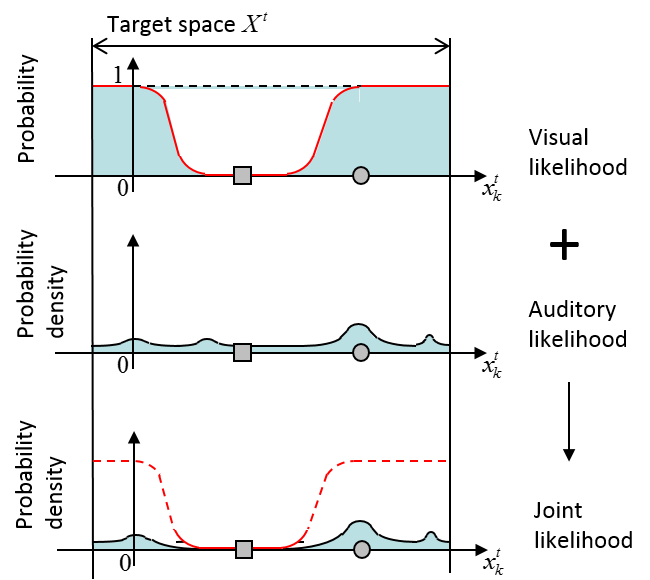
\includegraphics[height=60mm]{Figures/joint.png}
	}
	\subfigure[RBE incorporating an acoustic sensor]{
		\centering
		\label{fig:posterior}
		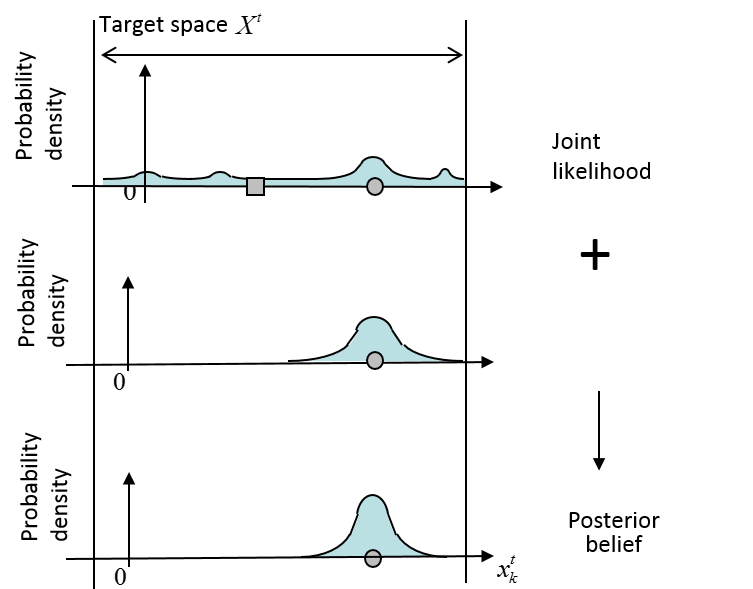
\includegraphics[height=60mm]{Figures/posterior.png}
	}
	\caption{Hybrid visual/auditory target estimation}
	\label{fig:hybrid}
\end{figure}

%%%%%%%%%%% begin figure %%%%%%%%%%%%%%%%%%%
\begin{figure}[h]
	{\centering
		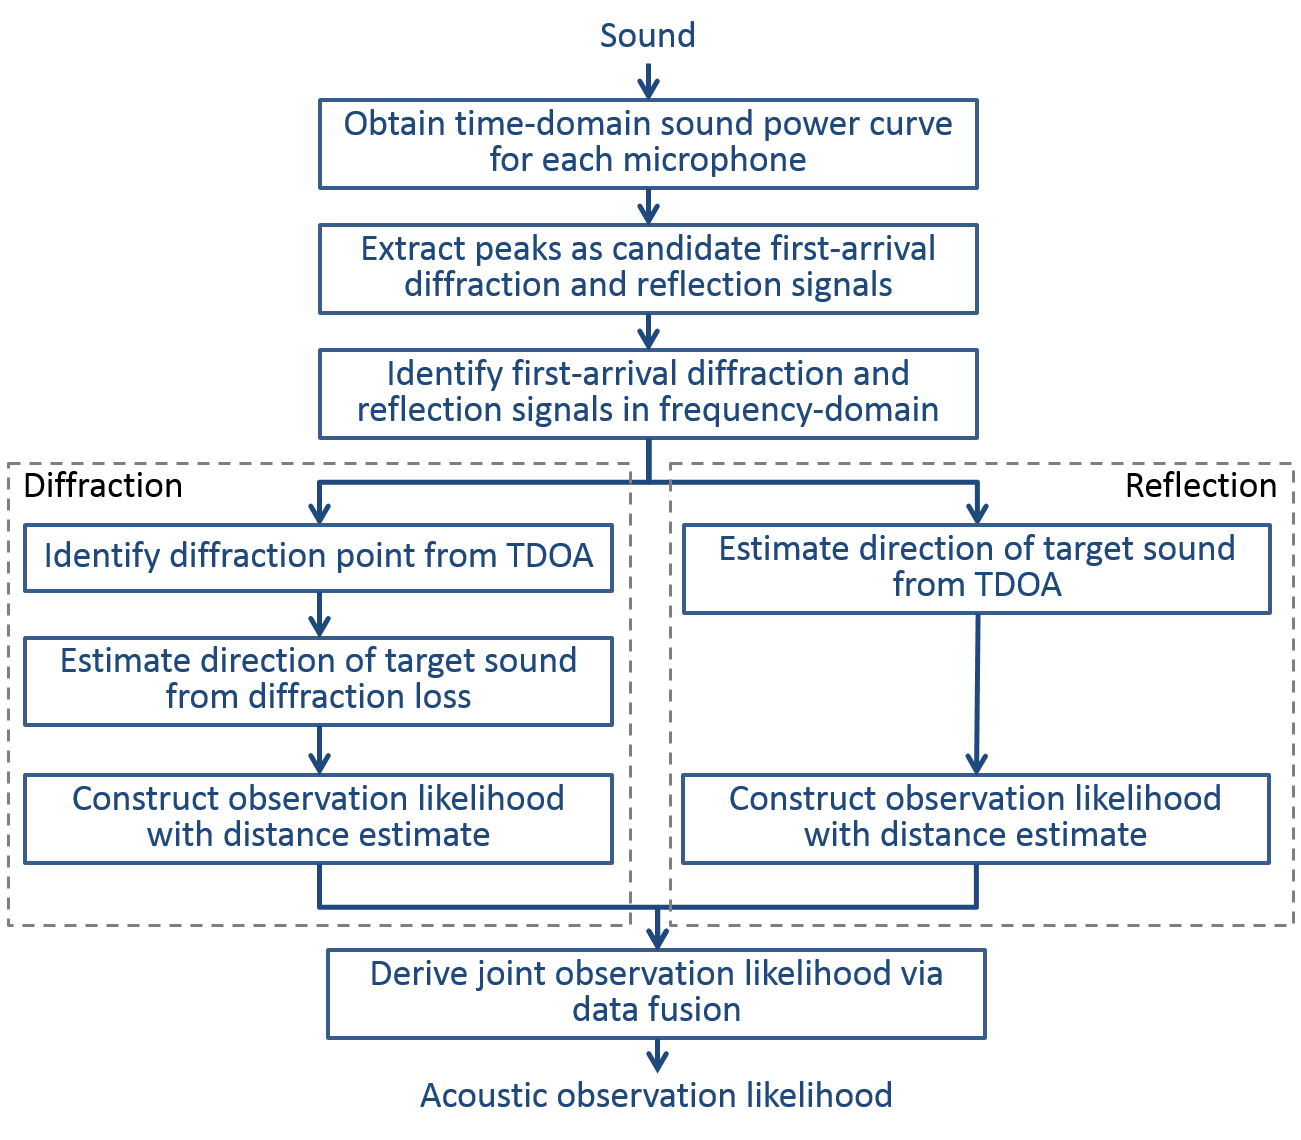
\includegraphics[height=0.40\textwidth]{Figures/auditory_procedure.png}
	}
	\caption{\footnotesize {Construction of auditory NFOV target likelihood} }
	\label{fig:auditory_procedure}
\end{figure}
%%%%%%%%%%%%%%%% end figure %%%%%%%%%%%%%%%%%%%
While the derivation of $\lia{\cdot}$ is most challenging and thus will be dealt with separately in the next section, the advantage of Equation (\ref{eq:joint}) in RBE is illustratively shown in Figure \ref{fig:hybrid}.  The possible locations of the target are narrowed down even though the no-detection likelihood is used in visual sensing since the likelihood clears out the joint likelihood in the FOV and dropped some peak(s) as shown in Figure \ref{fig:joint}. Because sharpest and most Gaussian is the visual observation likelihood with detection, the prior belief is most determined by the last visual observation and remains a sharp Gaussian distribution as shown in Figure~\ref{fig:posterior}.  The posterior belief with the joint observation likelihood inherits this characteristics since the joint likelihood most likely captures the target location with a peak and magnifies the confidence of the prior belief with the joint likelihood.  


\subsubsection{Construction of Auditory NFOV Target Observation Likelihood}

\noindent {\bf Overview}: Unlike the conventional techniques, the proposed approach 
\begin{itemize}
	\item Is not based on the LOS assumption and actively utilizes the physics of sound wave propagation associated with NFOV targets; 
	\item Does not need information such as the time of sound emission and power to be informed by the target;
	\item Does not need to collect acoustic cues in advance. 
\end{itemize}

Figure~\ref{fig:auditory_procedure} shows the overview of the approach proposed for constructing a NFOV target observation likelihood using an auditory sensor.  The core of the proposed approach is to extract the first-arrival diffraction and reflection signals by taking the physics of sound wave propagation into account.  Unlike radio signals, sound signals reflect significantly without penetrating into different media while they also diffract at low frequencies \cite{bellusci2007ultra}.  The proposed approach begins with obtaining a time-domain signal of a relatively impulsive sound at each microphone.  In each curve, notable peaks are then extracted as candidate first-arrival diffraction and reflection signals.  When each candidate signal is described in the frequency domain, the first-arrival diffraction and reflection signals can be identified since they are the first signals that are correlated in low frequency range.  The diffraction signal is then used to identify the so-called diffraction point by deriving the Time-Difference-Of-Arrival (TDOA) for each pair of microphones and further estimate the direction of target sound beyond the diffraction point from the loss of sound energy through diffraction, or the diffraction loss.  An observation likelihood is eventually constructed by additionally estimating the distance from the sound magnitude and characteristics.  The reflection signal estimates the target direction directly from the TDOA by mirroring and creating a virtual target.  It also creates an observation likelihood with distance estimate by considering sound magnitude and characteristics and environmental properties.  A joint observation likelihood is finally created by the fusion of the diffraction and reflection observation likelihoods.  

\begin{figure}[ht]
	\centering
	\subfigure[Acoustic signals from NFOV target]{
		\centering
		\label{fig:NFOV_acoustic}
		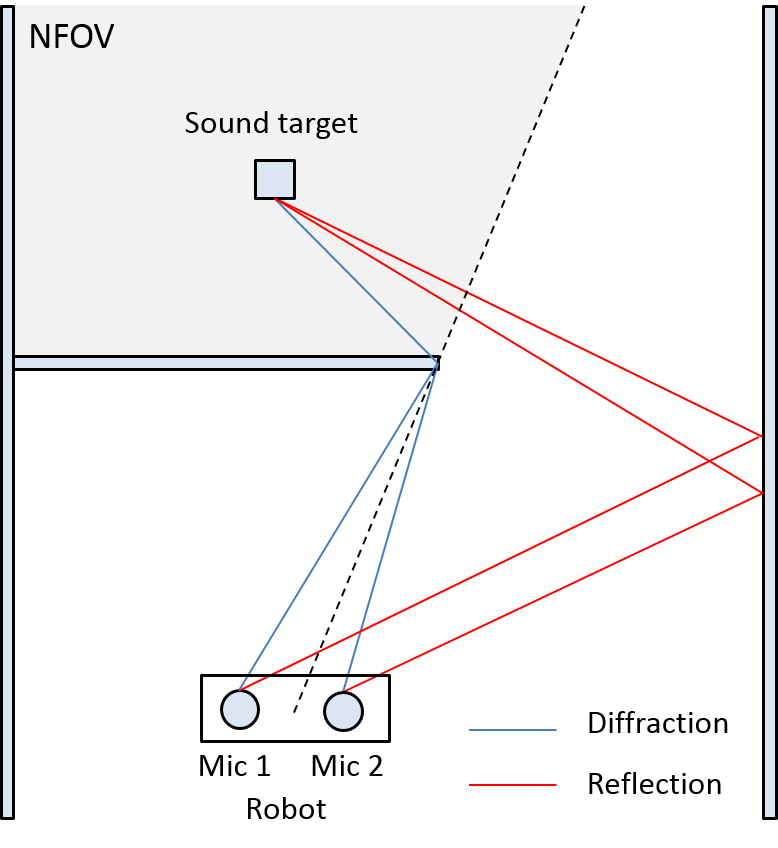
\includegraphics[height=60mm]{Figures/NFOV_acoustic.png}
	}
	\subfigure[Diffracted and reflected signals]{
		\centering
		\label{fig:sound_extraction}
		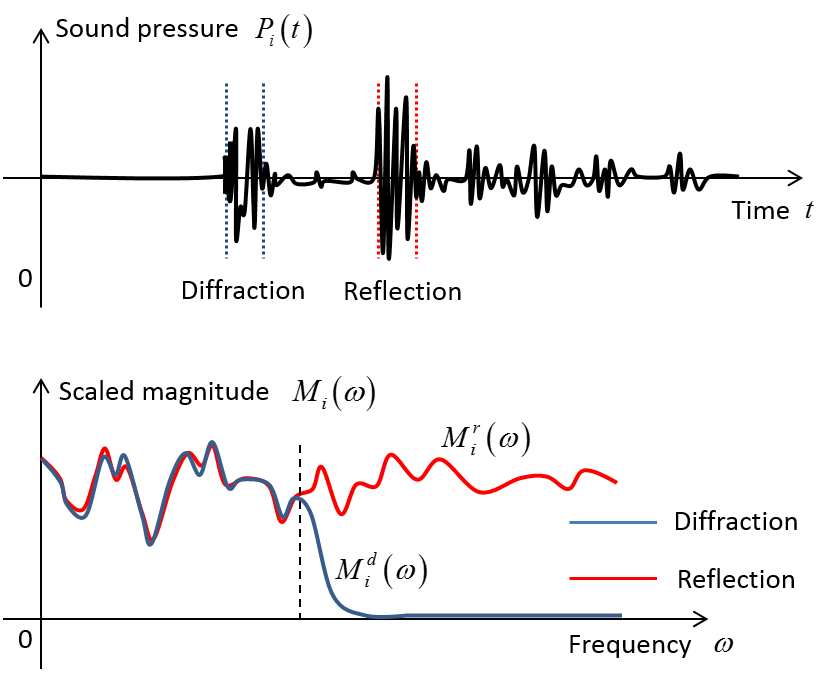
\includegraphics[height=50mm]{Figures/sound_extraction.png}
	}
	\caption{Auditory NFOV target observation}
	\label{fig:auditory_approach}
\end{figure}

The proposed approach infers the location of the sound target using both the first-arrival diffracted and reflected sound signals.  The next subsection describes the extraction of the first-arrival diffraction and reflection signals, followed by the target estimation using the diffracted and reflected signals in the subsequent two subsections.  The final goal of this project is to develop a probabilistic RBE based framework, but the preliminary study has succeeded in the proof-of-concept in deterministic formulations.  The two subsections will present the deterministic NFOV target estimation using diffraction and reflection sound waves.  The final subsection derives the joint observation likelihood as a result of data fusion.  

\section{Extraction of First-arrival Diffraction and Reflection Signals} 
Figure~\ref{fig:auditory_approach} shows the extraction process of the diffraction and reflection signals proposed in this project illustratively in one of the simplest scenarios where a robot carrying two microphones receives sound emitted by a target in the NFOV in a two-dimensional indoor environment with three walls (Figure~\ref{fig:NFOV_acoustic}).  As shown in the figure, sound waves emitted from the target reach the robot first through diffraction and second through reflection and, if the sound is relatively impulsive, the first-arrival diffraction and reflection signals can be extracted clearly.  Extraction becomes challenging for complex environments, but various existing techniques proposed to extract signals or select thresholds for extraction reportedly achieve successful extraction and identify candidate diffraction and reflection signals \cite{lee2006large,irahhauten2006investigation,xu2008delay,Guvenc2009}.  Figure~\ref{fig:sound_extraction} shows not only the sound pressure of sound in the time domain, $P_i\bs{t}$, but also the magnitude of the resulting first-arrival diffraction and reflection signals in the frequency domain, $M_i^d\bs{\omega}$ and $M_i^r\bs{\omega}$, where $i \in \bm{1,2}$ is the index of microphone.  Note that the magnitude is scaled to examine correlation.  Signals are considered from the same sound source if they share the same characteristics in low frequency because low-frequency signals reflect and diffract.  The proposed approach thus select the first set of signals that have the same low-frequency characteristics but are dissimilar in high frequency as the first-arrival diffraction and reflection signals of all the candidate signals.  Diffraction signals have little high-frequency components whilst reflection signals see components in all frequencies.  Needless to say, each of Microphones 1 and 2 constructs a different data set.  



%%%%%%%%%%% begin figure %%%%%%%%%%%%%%%%%%%
\begin{figure}[ht]
	\centering
	\subfigure[Proposed approach]{
		\centering
		\label{fig:diffraction1}
		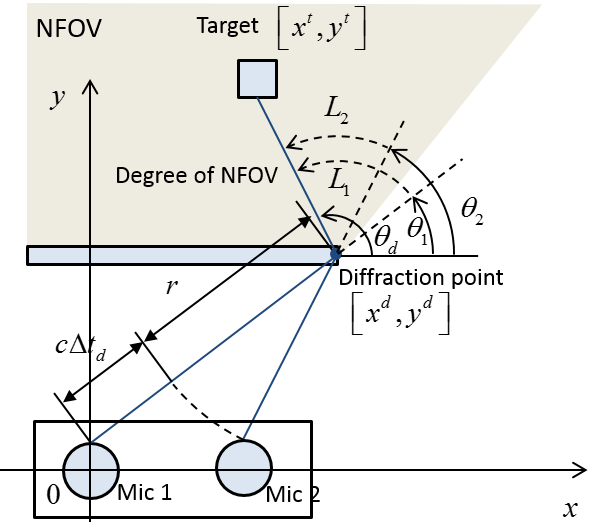
\includegraphics[height=50mm]{Figures/diffraction1.png}
	}
	\subfigure[Magnitude with different orientation angles \cite{medwin1981shadowing}]{
		\centering
		\label{fig:diffraction2}
		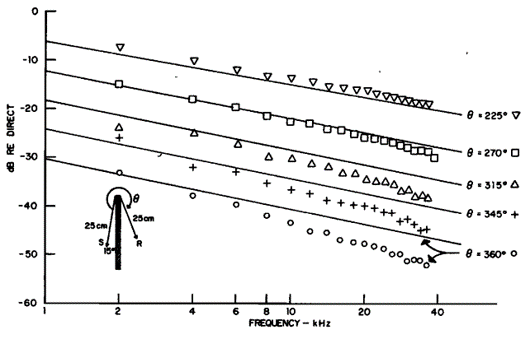
\includegraphics[height=50mm]{Figures/diffraction.png}
	}
	\caption{\footnotesize {Estimation of sound direction from diffraction signals} }
	\label{fig:diffraction}
\end{figure}
%%%%%%%%%%%%%%%% end figure %%%%%%%%%%%%%%%%%%%
\noindent {\bf Estimation of Sound Direction from Diffraction Signals}: Figure~\ref{fig:diffraction1} shows the notations used for target estimation from diffraction signals in the scenario introduced in the last subsection.  Since the diffraction sound Microphones 1 and 2 receive is originated from the LOS location at which the sound diffracts, the proposed approach starts target estimation from diffraction signals with the selection of diffraction point from all candidates, which are corners of all structures.  The measured quantity used for the selection is the TDOA, $\Delta t_d = t_{d2} - t_{d1}$, where $t_{d1}$ and $t_{d2}$ are the Times-of-Arrival (TOAs) at Microphones 1 and 2 respectively.  The diffraction point can be easily found from candidates as it satisfies the following equation:  
\begin{equation}\label{eq:TDOA1}
\bs{x^d}^2 + \bs{x^d}^2 = \bs{c \Delta t_d + r}^2.  
\end{equation}
where $\bl{x^d, y^d}$ is the location of a candidate diffraction point, $c$ is the speed of sound and $r$ is a shorter distance between a microphone and the candidate diffraction point.  
With the diffraction point identified, the proposed approach further identifies the direction of the sound target from the diffraction point by analyzing the magnitudes of diffraction and reflection sounds $M_i^d\bs{\omega}$ and $M_i^r\bs{\omega}$.  The loss of high-frequency signal components is assumed to be less with a microphone closer to LOS (Microphone 2 in this case) as there is no loss with a microphone on the LOS to the sound target.  This assumption, in fact, has been found to be valid by the work of Medwin a quarter-century ago \cite{medwin1981shadowing} shown in Figure~\ref{fig:diffraction2}.  The magnitude of diffraction sound drops when the ``degree of NLOS'' represented by the orientation angle is increased.   This makes the proposed approach define the diffraction loss as
\begin{equation}\label{eq:loss}
L_i = \int \bl{M_i^r\bs{\omega} - M_i^d\bs{\omega}} {\rm d} \omega \geq 0, \forall i \in \bm{1,2}  
\end{equation}
and associate it with the degree of NLOS.  The work of Medwin also shows that the diffraction loss is approximately proportional to the degree of NLOS.  The sound direction from the diffraction point is given by
\begin{equation}\label{eq:direction_diffraction}
\theta_d = \theta_1 + \frac{\theta_2 - \theta_1}{L_1 - L_2} L_1.   
\end{equation}
\noindent {\bf Estimation of Sound Direction from Reflection Signals}: Figure~\ref{fig:reflection} shows the proposed approach for estimation of sound direction from reflection signals.  Reflection makes the sound propagation and the subsequent target estimation complicated, but if the wall is smooth and yields specular reflection, the sound direction can be estimated easily by introducing a virtual target \cite{pulkki1997}, which is located symmetrically to the real target relative to the wall of reflection.  Let the position of the virtual target be $\bl{\hat x^t, \hat y^2}$.  The measured TDOA can be associated with the position of the virtual target as\\
%%%%%%%%%%% begin figure %%%%%%%%%%%%%%%%%%%
\begin{figure}[h]
	{\centering
		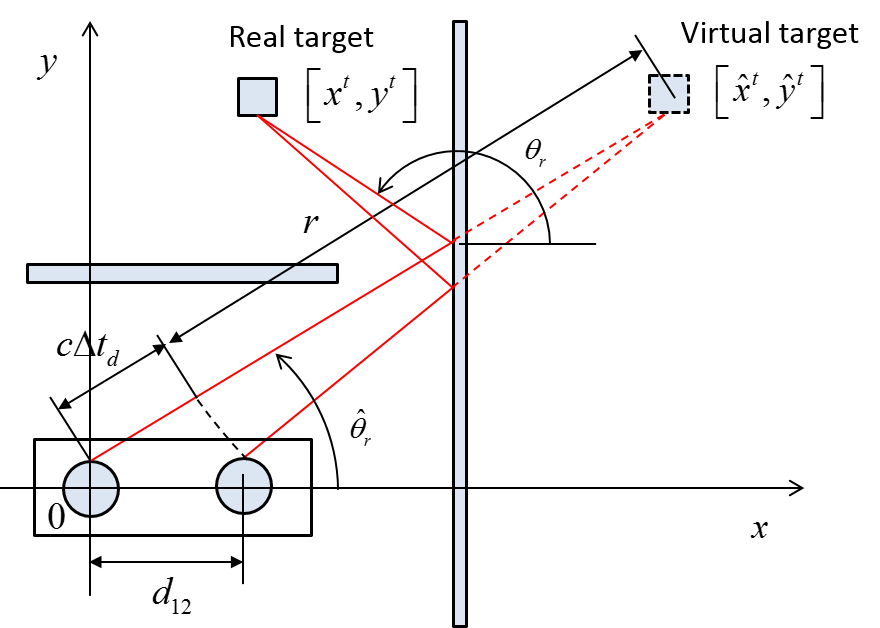
\includegraphics[width=0.35\textwidth]{Figures/reflection.png}
	}
	\caption{\footnotesize {Estimation of sound direction from reflection signals by proposed approach} }
	\label{fig:reflection}
\end{figure}
%%%%%%%%%%%%%%%% end figure %%%%%%%%%%%%%%%%%%%
\begin{equation}\label{eq:reflection}
\left\{
\begin{array}{ll}
\bs{\hat x^t}^2 + \bs{\hat y^t}^2 = \bs{r + c \Delta t_d}^2\\
\bl{\bs{\hat x^t}^2 - d_{12}}^2 + \bs{\hat y^t}^2 = r^2
\end{array},
\right.
\end{equation}
where $d_{12}$ is a distance between Microphones 1 and 2.  Since $r$ is unknown unlike the diffraction, the two equations with three unknowns, $\hat x^t$, $\hat y^t$ and $r$, introduce the relationship between $\hat x^t$ and $\hat y^t$ through the elimination of $r$.  Derivation attempted as a preliminary study for this project yields the relationship as
\begin{equation}\label{eq:estimation_reflection}
\bs{\hat y^t}^2 = \bs{\frac{d_{12}^2}{c^2 \Delta t^2} - 1} \bs{\hat x^t}^2 - d_{12} \bs{\frac{d_{12}^2}{c^2 \Delta t^2} - 1} \hat x^t + \bl{\frac{\bs{d_{12}^2 + c^2 \Delta t_d^2}}{4 c^2 \Delta t^2} - d_{12}^2}.  
\end{equation}
The further mathematical manipulation shows that this equation asymptotically yields the sound direction as 
\begin{equation}\label{eq:dirction_reflection}
\theta_r = \pi - \hat \theta_r = \lim_{r \rightarrow \infty} \tan^{-1} \frac{\hat y^t}{\hat x^t}= \cos^{-1} \frac{c \Delta t_d}{d_{12}}.   
\end{equation}
%%%%%%%%%%% begin figure %%%%%%%%%%%%%%%%%%%
\begin{figure}[h]
	\centering
		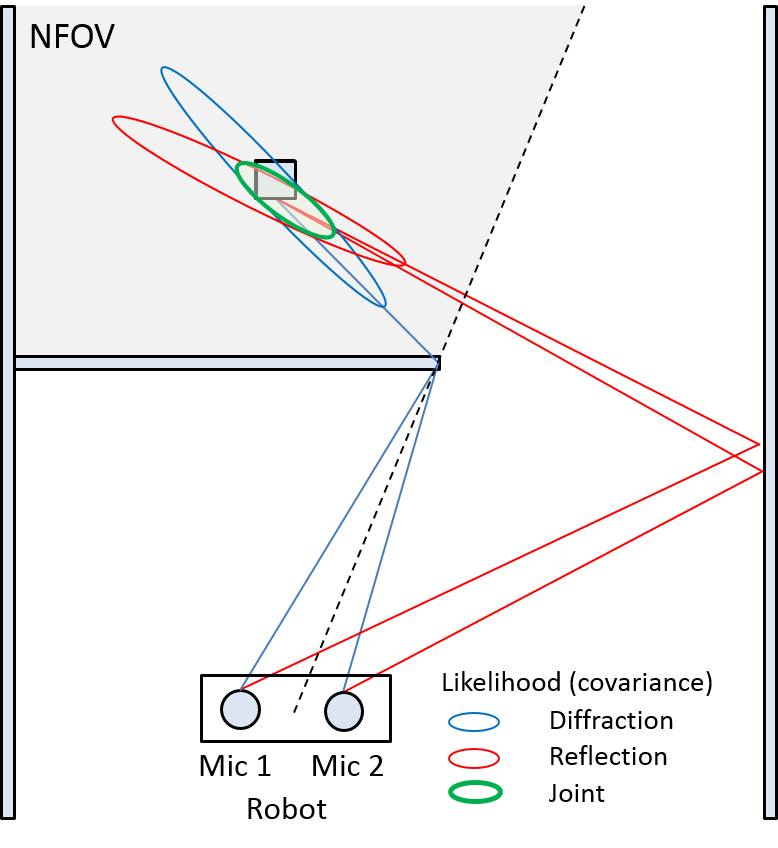
\includegraphics[width=0.30\textwidth]{Figures/data_fusion.png}
	\caption{\footnotesize {Construction of joint observation likelihood through data fusion} }
	\label{fig:data_fusion}
\end{figure}
%%%%%%%%%%%%%%%% end figure %%%%%%%%%%%%%%%%%%%
\noindent {\bf Construction of Joint Observation Likelihood through Data Fusion}: 
While the sound can be better identified in direction rather than distance, it is also possible to make an estimate on how far the sound target is.  The proposed approach makes the estimate by utilizing any available information including the magnitude, sound patterns stored in a database, or sound characteristics in a knowledge base and constructs an observation likelihood for each of the diffraction and reflection signals by modeling uncertainties.  For the $j$th pair of microphones, the diffraction and reflection likelihoods are then combined to create an auditory joint observation likelihood via the canonical data fusion formula: 
\begin{equation}\label{eq:joint_auditory}
\lia{\Vxbp{k}{t}|\ptVzbp{s}{k}{t},\mVxbp{k}{s},\mVmb{k}} = \lid{\Vxbp{k}{t}|\ptVzbp{s}{k}{t},\mVxbp{k}{s},\mVmb{k}} \lir{\Vxbp{k}{t}|\ptVzbp{s}{k}{t},\mVxbp{k}{s},\mVmb{k}} 
\end{equation}
where $\lid{\cdot}$ and $\lir{\cdot}$ are the diffraction and reflection observation likelihood.  
Figure~\ref{fig:data_fusion} illustrates the diffraction and reflection observation likelihoods as well as the joint observation likelihood where the observation likelihood is represented by an ellipsoid indicating a probability distribution with a covariance.  The diffraction and reflection likelihoods are shown to have high eccentricity due to more accuracy in direction than in distance.  Since the difference of the diffraction and reflection likelihoods in orientation may not be significant, the resulting auditory joint likelihood could also given by an ellipsoid with high eccentricity, but the proposed approach, utilizing the diffraction and reflection physics of sound, could estimate the location of the sound target.  
%=================================================================


\begin{table}[h]
\caption{An Example of a Table}
\label{table_example}
\begin{center}
\begin{tabular}{|c||c|}
\hline
One & Two\\
\hline
Three & Four\\
\hline
\end{tabular}
\end{center}
\end{table}


   \begin{figure}[thpb]
      \centering
      \framebox{\parbox{3in}{We suggest that you use a text box to insert a graphic (which is ideally a 300 dpi TIFF or EPS file, with all fonts embedded) because, in an document, this method is somewhat more stable than directly inserting a picture.
}}
      %\includegraphics[scale=1.0]{figurefile}
      \caption{Inductance of oscillation winding on amorphous
       magnetic core versus DC bias magnetic field}
      \label{figurelabel}
   \end{figure}

\section{Numerical Analysis}
The preliminary experimental study has demonstrated validity of the proposed approach through simulation.




\section{CONCLUSIONS}
\addtolength{\textheight}{-12cm}   % This command serves to balance the column lengths
                                  % on the last page of the document manually. It shortens
                                  % the textheight of the last page by a suitable amount.
                                  % This command does not take effect until the next page
                                  % so it should come on the page before the last. Make
                                  % sure that you do not shorten the textheight too much.
                                  
\bibliographystyle{ieeetran}            
\bibliography{References/cite_cur}   % name your BibTeX data base
%%%%%%%%%%%%%%%%%%%%%%%%%%%%%%%%%%%%%%%%%%%%%%%%%%%%%%%%%%%%%%%%%%%%%%%%%%%%%%%%
%%%%%%%%%%%%%%%%%%%%%%%%%%%%%%%%%%%%%%%%%%%%%%%%%%%%%%%%%%%%%%%%%%%%%%%%%%%%%%%%
%%%%%%%%%%%%%%%%%%%%%%%%%%%%%%%%%%%%%%%%%%%%%%%%%%%%%%%%%%%%%%%%%%%%%%%%%%%%%%%%
%\section*{APPENDIX}
%Appendixes should appear before the acknowledgment.
%\section*{ACKNOWLEDGMENT}
%%%%%%%%%%%%%%%%%%%%%%%%%%%%%%%%%%%%%%%%%%%%%%%%%%%%%%%%%%%%%%%%%%%%%%%%%%%%%%%%
\end{document}